% Official template of the Research Group COMPUTATIONAL SOCIAL SCIENCE AND SYSTEMS ANALYTICS
% If you have problems after you did not find a solution on Stack Overflow or similar websites, or if you have an idea on how to improve this template,
% you can contact the author of the template: janina.lsd@uni-muenster.de

% ============================================================

% xxxxxxxxx  FIRST ADJUST THE FOLLOWING OPTIONS xxxxxxxxx
% a) the language of your thesis to either "english" or "german",
% b) the type of the thesis to either "bachelor", "master" or "seminar",
% c) and if the supervisor is equal to the principal supervisor
    % d1) It is possible that your thesis is supervised only by a member of the institute with a doctor title and no supervising professor. Then, you can use "postdoc" --> e.g., Dr. Lechtenbörger, ...
    % d2) else if there is a professor and a supervisor use "supervisor".
% d) If you are writing a thesis jointly with other students, set it to true for (seminar) paper with multiple authors.

\documentclass[
    language=german, % german english
    thesis=bachelor, % seminar bachelor master
    supervisor=postdoc, % supervisor postdoc
    multiauthor=false, % true false 
    ]{settings/csssa-thesis}

% ============================================================
% Include all relevant information for the title page

\title{Title of an Awesome Thesis Which Will Change the World and Reveal Incredible Insights Into Highly Relevant Topics}
% If multiple authors write a (seminar) paper, use commas or newline (\\) to separate names, e-mail addresses, ids. Examples are given as comments below. 
\author{First Middle Lastname}
%\author{Maja Mustermann, Max Musterfrau} \author{First Middle Last Name\\Second Student with somewhat longer Name}
\email{student@uni-muenster.de}
% Matriculation Number
\id{123456}
% Information about the thesis and the course
\professor{Dr. Professor}
\supervisor{Supervisor, M.Sc.}
% You only have to include the course if you are writing a seminar thesis
\course{Super interesting seminar}
% Submission Date
\date{01.01.2025}

% ============================================================


% ============================================================
% Place for adding additional packages (if required)
% 
% 
  
% ============================================================


% ============================================================
\begin{document}
\maketitlepage
\maketitle

\begin{abstract}
    \lipsum[1]
\end{abstract}

\section{Introduction}

Welcome! This document serves to characterize the guidelines for crafting and formatting seminar papers, Bachelor's, and Master's theses. It will inform about the general formatting rules applicable to any written submission, alongside demonstrating how the provided \LaTeX\ template can facilitate the creation of a well-formatted document. Throughout this guide, several examples will elucidate the academic work's structure while showcasing the template's utilization. However, it's important to note that while this guide covers many aspects of paper writing and achieving an aesthetically pleasing outcome, it cannot encompass all possible considerations. For further details on seminar participant expectations, please consult your supervisors or guides online.

This template comprises a \texttt{main.tex} file merging all components. Within the \texttt{code} folder, you can integrate algorithm and code block files pertinent to the thesis. According to your liking, in the \texttt{content} folder, each relevant section can be included as individual \texttt{tex} files. As implied by its name, the \texttt{figures} folder is designated for images and graphics inclusion. It is recommended not to modify the \texttt{settings} folder. Should you need to incorporate additional packages not provided by this template, you can do so in the preamble of \texttt{main.tex}.

\section{Template Manual}\label{ch02:manual}

Below, you'll find some general information on utilizing this template, along with tips on leveraging various features of \LaTeX\ to craft not only a comprehensive but also well-structured thesis. This isn't intended as a comprehensive manual for learning \LaTeX, but rather as a reminder of certain features and a guiding resource.

One crucial tip: strive to avoid situations where only one or one and a half lines of a paragraph spill onto the next page. These fragmented sections can easily be overlooked by your reader and detract from the elegance of typesetting. Occasionally, \LaTeX\ may incorrectly separate words or push them to the margins of the page if they're unfamiliar. Utilize the \combrac{hyphenation}{com-mand} in the preamble of the \texttt{main.tex} file to instruct \LaTeX\ on proper word separation.

\subsection{Text Structure}\label{ch02:sec1:structure}

When structuring an academic work, particularly concerning the criterion of \emph{completeness}, it's essential to maintain coherence. Achieving completeness should not entail redundancies or overlaps. The entire work should adhere to a central theme, with each section, and even each argument, logically progressing within this thematic framework. Moreover, this theme should be readily apparent to readers, who should be able to discern their position within the argument at any given point. Employing a continuous example throughout the writing process can facilitate this coherence.

In this thesis, conventional structures such as \com{chapter}, \com{section}, and \com{subsection} can be utilized. Depending on the thesis's length, it's advisable not to exceed these three subdivisions. When referring to chapters, employ the \combrac{label}{label} and related \combrac{ref}{label} commands. For instance, write \verb|see Chapter~\ref{ch02:manual}| rather than \verb|see \ref{ch02:manual}|. (The same principle applies to tables, figures, etc.: Clearly state the type of reference, capitalize it, and use the tilde character to create a non-breaking space before the number.)

In \LaTeX, various commands such as \combrac{textit}{text} for italics, \combrac{textbf}{text} for bold text, \combrac{textsc}{text} for small caps, \combrac{underline}{text} for underlined text, or \combrac{texttt}{text} for typewriter text can be employed to emphasize information. However, it's advisable to use a limited number of highlighting styles and maintain consistency by sticking to one type of highlight for a specific purpose.

Texts can also be structured using lists. Common list environments like \texttt{itemize}, \texttt{enumerate}, and \texttt{description} are compatible with this template and can aid in organizing content effectively.

\subsection{Colours}\label{ch02:sec2:color}

This template comes with the colors defined in the Corporate Design of the University of Münster and ERCIS. Table~\ref{sec2:tab:colors} lists the color names and shows the resulting color. You can apply them to text by using the \combrac{textcolor\{color name\}}{text} command. If you want to use them in other images or graphics, you will also find the hexadecimal codes below. Do not forget to add an \# before you use them in other applications.

\begin{table}[H]
    \centering
    \caption{Representation of color codes defined in this template.}
    \label{sec2:tab:colors}
    \begin{tabular}{@{}lcc@{}}
        \toprule
        \textbf{Color Name} & \textbf{Result} & \textbf{Hex Code} \\ \midrule
            um-black     & \textcolor{um-black}{\blacksmiley{}} & 3e3e3b \\
            um-lightgreen  & \textcolor{um-lightgreen}{\blacksmiley{}} & 7ab516 \\
            um-green      & \textcolor{um-green}{\blacksmiley{}} & 008e96 \\
            um-lightblue      & \textcolor{um-lightblue}{\blacksmiley{}} & 009dd1 \\
            um-blue     & \textcolor{um-blue}{\blacksmiley{}} & 006e89 \\
            ercis-red      & \textcolor{ercis-red}{\blacksmiley{}} & 852339 \\
			\bottomrule
    \end{tabular}
\end{table}

\subsection{Floats}\label{ch02:sec3:floats}

In order to include float objects, the usual commands for inserting a   \texttt{table}, \texttt{figure} or \texttt{listing} / \texttt{algorithm} can be used. For figures, tables as well as code, proper captions, and labels should be set. Similar to chapters and sections, labels can be set to refer to the floating object. Captions should help the reader what kind of information is displayed as well as why is it displayed. This template does not include a list of figures or a list of tables. Again, please keep in mind that these missing lists are missing on purpose and should only be included in this template if your supervisor asks for it.

Additionally, you can determine where images and tables should be placed on the page. In scientific publications, it is the state-of-the-art to place them on top of the page. If it fits in your case, you should also stick to this rule of thumb. Use the square brackets after the definition of the environment to force \LaTeX{} to place the floats where you want them to be: \texttt{h} for here, \texttt{t} for at the top of the page and \texttt{b} for the bottom of the page. You can also combine them in order to give \LaTeX{} some margin for maneuver.

Tables need nested environments. First, a \combrac{begin}{table} environment is used, in which a \combrac{begin}{tabular} environment is called. See Table~\ref{sec2:tab:colors} for an example. The \texttt{tabular} environment is used to define the table itself. Please make sure that all information is structured properly so that the reader can directly see and understand the displayed information. A guide for really nice tables can be found in the documentation of the \texttt{booktabs} package which is also included in this template \citep{Fear2020booktabs}.


% Merged with the DBIS template (Section 2.5.2)
For included images, make sure to use high-resolution images (vector) images or that you generate images by using the \texttt{TikZ/PGF} package in \LaTeX, the \texttt{ggplot} package in \texttt{R} or the \texttt{seaborn} package in \texttt{python}. They can be included by placing them in a \verb|\begin{figure}|-environment and by using the \combrac{includegraphics[width]}{file} command, which can handle many formats. PDF files are preferable for vector graphics.  PNG files are the best way of including pixel graphics, such as graphs or diagrams not available in vector format.  JPEG files may be used to include photographic or artistic images.

\begin{figure*}[ht]
    \centering
    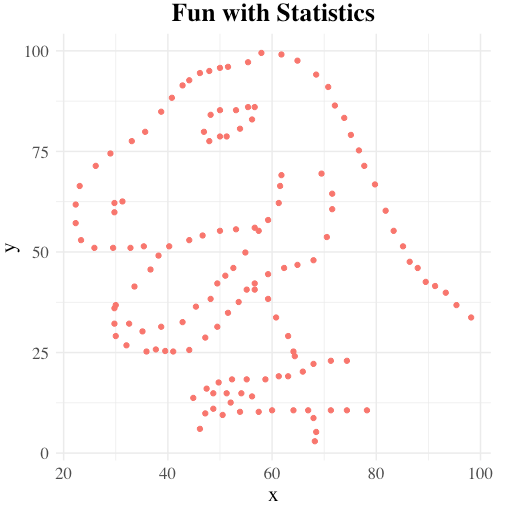
\includegraphics[width=0.6\textwidth]{figures/dummy_figure.png}
    \caption{Always choose a proper label and caption which describes what the reader can see. You should write complete sentences and not only keywords. This nice image was generated by using the \texttt{ggplot}-package of \texttt{R}.}\label{fig:my_label}
\end{figure*}

The last type of float which can be included are code snippets. You can either include pseudocode to outline the mechanisms of algorithms or real source code.

Pseudocode should be created by using the \texttt{algorithmicx} package. It provides some commands to structure the code and is easy to handle. As tables, the outer environment is the \texttt{algorithm} environment, while the inner environment is an \texttt{algorithmic}-environment. Further information on how to use the commands can be found in the documentation of the \texttt{algorithmicx} package \citep{Janos2020algorithmicx}.

\begin{algorithm}
    \begin{algorithmic}[1]
        \Procedure{Euclid}{$a,b$} \Comment{required b > a}
        \State $r\gets a\bmod b$
        \While{$r\not=0$}
              \State $a\gets b$
              \State $b\gets r$
              \State $r\gets a\bmod b$
           \EndWhile\label{euclidendwhile}
           \State \textbf{return} $b$
        \EndProcedure
    \end{algorithmic}
    \caption{Euclid’s algorithm in pseudo-code}\label{ch02:code:pseudo-euclid}
\end{algorithm}

For source code, the package \texttt{minted} is already included in this thesis. It provides features to highlight keywords in code for several programming languages. Simply  include code files via the \combrac{inputminted\{language\}}{file} command in a \texttt{listings} or \texttt{algorithm} environment. If it is just one single line, use \combrac{mint}{language}\texttt{|Line of Code|}.

Be aware that if you want to use the \texttt{minted} package on your local computer and not in Overleaf, you might have to install some packages on your local machine. For further information, take a look at the package documentation \citep{Poore2020minted}.\label{ch02:sec3:minted}

\begin{algorithm}[ht]
    \inputminted[
    xleftmargin=20pt,
    framesep=2mm,
    baselinestretch=1.2,
    linenos
    ]{python}{code/euclid.py}
    \caption{Euclid’s algorithm in python-code}\label{ch02:code:python-euclid}
\end{algorithm}

\subsection{Subfloats}

Sometimes it makes sense to place figures side by side. Use the \texttt{subfloat} environment inside a \texttt{figure} environment if you want to reference the images separately. If not, you can also use two commands without an additional environment by including two \combrac{includegraphics[width]}{image} commands and adjust the width so that the images are placed side by side. Note that the sizes of either the subfigures or the images should be together lower than 1, e.g., both \texttt{width=0.49\com{textwidth}}.

\begin{figure}[ht]
    \centering
    \begin{subfigure}{0.49\textwidth}
        \centering
        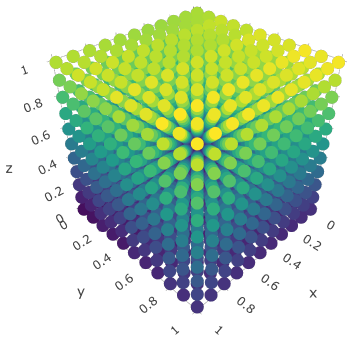
\includegraphics[width=0.8\textwidth]{figures/dummy-subfigure1.png}
        \caption{The caption of the first image.}\label{ch02:fig:fig1a}
    \end{subfigure}
    \begin{subfigure}{0.49\textwidth}
        \centering
        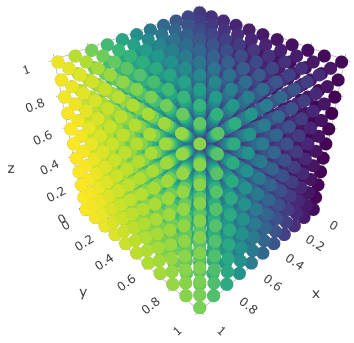
\includegraphics[width=0.8\textwidth]{figures/dummy-subfigure2.png}
        \caption{The caption of the second image.}\label{ch02:fig:fig1b}
    \end{subfigure}\label{ch02:fig:fig1}
    \caption{Two interesting figures side by side which can be referenced independently. These images were generated by using the \texttt{plotly} extension for \texttt{R}.}
\end{figure}

\subsection{Bibliography and Citations}

Bibliographies are an important part of any piece of academic writing. On the one hand they enable readers to easily extend research on the given work.  On the other hand they help writers to correctly address their sources as well as keeping track of them.  With \LaTeX{}, bibliographic information is managed in \texttt{.bib} files (e.g., see \texttt{library.bib} coming with this template).

\LaTeX{} provides several commands to reference sources, which are then included in the bibliography at the end of the document.  This template uses \href{http://ctan.org/pkg/biblatex}{biblatex} (with \texttt{biber} as backend) and the option \texttt{natbib}.  The style of references and bibliography depends on your setting of \texttt{chair} in the beginning of the main document.  Please make sure to set that option first.  Then, different variants of citation commands may look as follows (others exist as well):

Use authors as subject in proper English sentence. \combrac{textcite}{Goodfellow2016deep} define \ldots produces: \textcite{Goodfellow2016deep} define \ldots

\begin{itemize}
    \item Use authors as subject in proper English sentence. For instance, using the command  ``\combrac{textcite}{Goodfellow2016deep} define \ldots'' you can produce: ``\textcite{Goodfellow2016deep} define \ldots''
    \item Note how more than three authors are automatically replaced with “et al.”. ``\combrac{textcite}{Goodfellow2014gan} define \ldots'' produces: ``\textcite{Goodfellow2014gan} define \ldots''
    \item Use reference at end of sentence or as object:
      \begin{itemize}
      \item ``\ldots~\combrac{citep}{Goodfellow2014gan}.'' produces: ``\ldots~\citep{Goodfellow2014gan}.''
      \item ``as stated in~\combrac{citep}{Goodfellow2014gan}, \ldots'' produces: ``as stated in~\citep{Goodfellow2014gan}, \ldots''
      \end{itemize}
    \item Include page numbers, e.g., ``\combrac{citep[p.~2]}{Codd1970relational}'' produces: ``\citep[p.~2]{Codd1970relational}''
    \end{itemize}

Generally, each source has to be named and should also be used with the publishing year to differentiate different works by the same author. How this can be done varies between institutions and departments. Relevant literature can be included in the \texttt{library.bib} file in the main folder of this template. Inside, you will also find some examples on which information is needed for which type of literature.

If authors or book titles are mentioned by name, the source should be cited right after them, e.g.: The book \emph{Artificial Intelligence: A Modern Approach}~\citep{Rusell2003artificial} has been written by S. J.\ Russel and P.\ Norving.

Note that sources should \emph{not} just be listed at the end of a paragraph.  Instead, sources should be cited when they are used. For instance, the following sentence might be the first one in a paragraph on Generative Adversarial Networks: According to~\textcite{Goodfellow2014gan}, Generative Adversarial Networks share the following major advantages \ldots (followed by text based on that source). Also, note that when referencing sources, the references is placed \textit{before} the punctutation that ends the sentences. Place it after when you use quotes. 

\subsection{Headings}
As mentioned above, if a section is broken further down, at least two subheadings shall follow.

\subsubsection{Subheadings}
This means a structure like this is \emph{NOT} appreciated for this is the only subheading. Therefore, there is no need to have it in the first place.

\subsection[Blacklist]{Blacklist of commands and packages}
You can include packages in the preamble of the \texttt{main.tex}-file if you need more than already defined in this template. But below you will also find a list of packages which should not be included in this document since, e.g., some of them interfere with existing packages. Also, all packages and commands which alter the design of the thesis, margins, indents or any other spaces are especially forbidden.

Disallowed packages:
\begin{description}
    \item[\combrac{usepackage}{authblk}] This package changes the default settings of the title page.
    \item[\combrac{usepackage}{subfig}] This package interferes with the already loaded \texttt{float} package.
    \item[\combrac{usepackage}{fullpage}] This package interferes with the already loaded \texttt{geometry} package.
    \item[\combrac{usepackage}{grffile}] Use proper file names, then you do not need this package.
    \item[\combrac{usepackage}{wrapfig}] Text is not allowed to float around figures.
\end{description}

Disallowed commands:
\begin{description}
    \item[\textbackslash{}addtolength] You are not allowed to change any margins or other page styles.
    \item[\textbackslash{}baselinestretch] You are not allowed to change any margins or other page styles.
    \item[\textbackslash{}tiny] This is not an acceptable font size.
    \item[\textbackslash{}vspace] No negative value may be used in proximity of a caption, figure, table, section, subsection, subsubsection, or reference.
    \item[\textbackslash{}vskip] No negative value may be used to alter spacing above or below a caption, figure, table, section, subsection, subsubsection, or reference.
\end{description}


\printbibliography[heading=header]
\backmatter     

% ============================================================

\end{document}